\section{Hydrodynamik - Ideale Fluide}

\textbf{Ideale Fluide nehmen keine Scherkräfte auf (keine Reibung) und sind inkompressibel.}


\subsection{Stromlinien-Modell}

\begin{itemize}
	\item Stromlinien zeigen Geschwindigkeit des Fluids
	\item \textbf{Dichte} Stromlinien bedeutet \textbf{hohe} Geschwindigkeit
	\item \textbf{Dünne} Stromlinien bedeutet \textbf{niedrige} Geschwindigkeit 
	\item Stationär: Stromlinien schneiden sich nicht 
\end{itemize}


\subsection{Kontinuitätsgleichung}

\begin{center}
	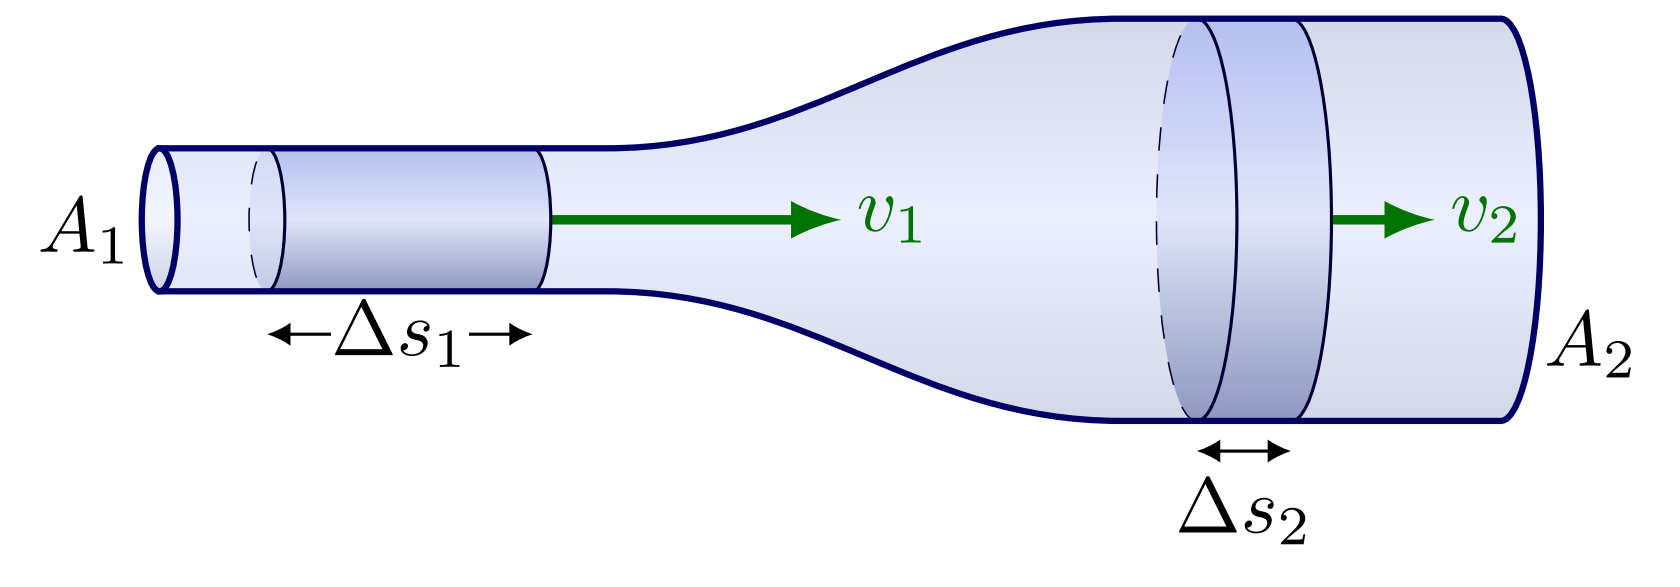
\includegraphics[width=0.7\columnwidth]{images/Kontinuitaet.png}
\end{center}

\vspace{-0.5cm}

$$ \boxed{ \frac{\Delta V}{\Delta t} = \dot{V} = A \cdot v = \const  \quad \Leftrightarrow \quad  A_1 \cdot v_1 = A_2 \cdot v_2 = \frac{\Delta V}{\Delta t} = \dot{V}} $$ 

\renewcommand{\arraystretch}{1.3}
\begin{tabular}{c l c}
	$\Delta V$	& Volumenänderung 					& $[\Delta V] = \meter^3$					\\
	$\Delta t$ 	& Zeitänderung 						& $[\Delta t] = \second$  					\\
	$\dot{V}$ 	& Volumenstrom (Volumen pro Zeit) 	& $[\dot{V}] = \frac{\meter^3}{\second}$	\\
	$A_x$ 		& Querschnittsfläche 				& $[A_x] = \meter^2$ 						\\
	$v_x$ 		& Geschwindigkeit der Flüssigkeit 	& $[v_x] = \frac{\meter}{\second}$
\end{tabular}
\renewcommand{\arraystretch}{1}

\medskip

\textrightarrow\ Gilt auch für Gase, wenn $v \ll v_{\rm Schall}$


\subsection{Bernoulli-Gleichung}

\begin{minipage}[c]{0.38\columnwidth}
	\raggedright
	Die Bernoulli-Gleichung beschreibt ein \myul{bewegtes} Fluid

	$$ \underbrace{ p + \rho \cdot g \cdot h }_{\substack{\mathrm{statisch}}} 
	+ \underbrace{ \frac{1}{2} \, \rho \cdot v^2 }_{\substack{\mathrm{dynamisch}}} = \const $$
	$$v = \frac{\Delta s}{t} \quad , \quad p = \frac{F}{A}$$
\end{minipage}
\hfill
\begin{minipage}[c]{0.6\columnwidth}
	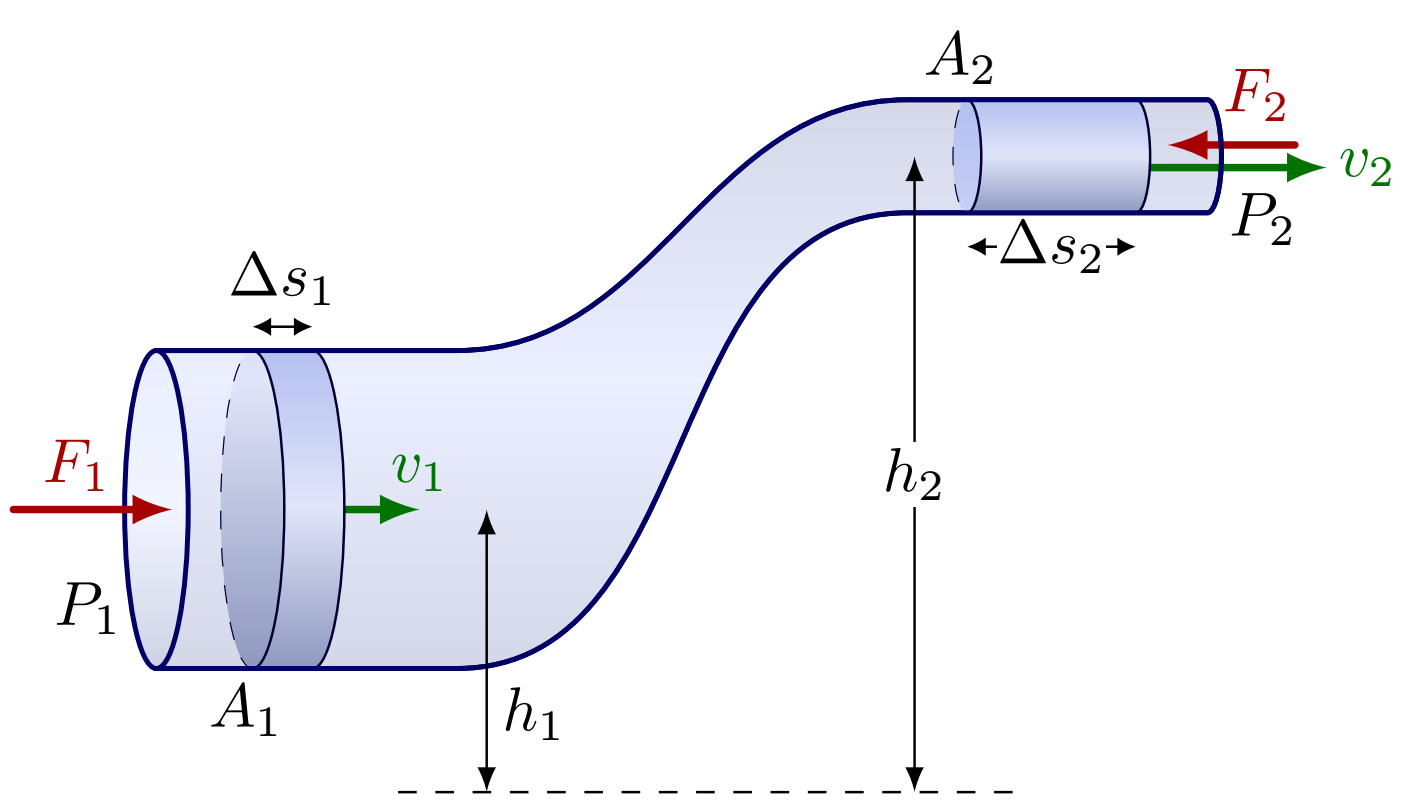
\includegraphics[width=\columnwidth]{images/Bernoulli.png}
\end{minipage}

\smallskip

$$ \boxed{ p_1 +  \rho \cdot g \cdot h_1 + \frac{1}{2} \, \rho \cdot v_1^2 = p_2 +  \rho \cdot g \cdot h_2 + \frac{1}{2} \, \rho \cdot v_2^2 } $$

\medskip


\begin{minipage}[t]{0.48\columnwidth}
	\subsubsection*{Spezialfall: Horizontal}

	$$ \boxed{ p + \frac{1}{2} \, \rho \cdot v^2 = \const } $$
\end{minipage}
\hfill
\begin{minipage}[t]{0.48\columnwidth}
	\subsubsection*{Spezialfall: Statik}

	$$ \boxed{ p + \rho \, \cdot g \cdot h =  \const} $$
\end{minipage}

\medskip


\subsubsection*{Hydrodynamisches Paradoxon}

\textbf{Je grösser die Strömungsgeschwindigkeit, desto kleiner der Druck} \\
\textrightarrow\ Gegen jede Intuition!

Se un estremità è aperta allora $p=0$ (ad Esempio in una siringa)

\subsubsection*{Formule derivate}

$$\dot{V} = \sqrt{\frac{2\Delta p}{\rho} \cdot \frac{A_1^2\cdot A_2^2}{A_1^2 - A_2^2}}$$

\subsection{Bernoulli-Gleichung und Energieerhaltung}

Die in der Bernoulli-Gleichung vorkommenden Terme können als \myul{Energie pro Volumen} betrachtet werden.

\vspace{-0.3cm}

\begin{align*}
	E_{\rm Mech}	&= \text{\color{orange}Elastische Energie } + \text{\color{violet}pot. Energie } + \text{\color{blue}kin. Energie} \\
					&= \cor{p \cdot V} + \cvt{m \cdot g \cdot h} + \cbl{\frac{1}{2} \, m \cdot v^2} = \const
\end{align*}

Wenn durch das Volumen dividiert wird erhält man: 

\vspace{-0.3cm}

\begin{align*}
	\frac{E_{\rm Mech}}{\text{Volumen}}	&= \frac{\text{elatische Energie}}{\text{Volumen}} + \frac{\text{pot. Energie}}{\text{Volumen}} + \frac{\text{kin. Energie}}{\text{Volumen}} \\
										&= p + \rho \cdot g \cdot h + \frac{1}{2} \, \rho \cdot v^2 = \const
\end{align*}

Bei einer horizontalen Strömung entfällt die pot. Energie (pro Volumen)

\vspace{-0.3cm}

\begin{align*}
	\frac{E_{\rm Mech}}{\text{Volumen}}	&= \frac{\text{elatische Energie}}{\text{Volumen}} + \frac{\text{kin. Energie}}{\text{Volumen}} \\
										&= p + \frac{1}{2} \, \rho \cdot v^2 = \const
\end{align*}

\subsection{Kraft auf rohr}
Viene utilizzato il simbolo $\vec{I}$ per l'impulso  per evitare confusione con la pressione $p$.

\subsubsection{Principi Fondamentali}
\begin{itemize}
    \item \textbf{Solidi:} $\vec{I} = m \cdot \vec{v}$ La variazione temporale dell'impulso corrisponde alla forza: $\frac{d\vec{I}}{dt} = \vec{F}$
    \item \textbf{Fluidi (Volume di controllo):} L'impulso totale in un volume $V$ è definito come:
    $$\vec{I} = \iiint_V \rho \cdot \vec{v} \, dV$$
    \item \textbf{Equazione della conservazione:} La somma delle forze esterne è pari alla variazione del flusso di quantità di moto:
    $$\sum \vec{F} = \frac{d\vec{I}}{dt}$$
\end{itemize}

\subsubsection{Bilancio dell'Impulso (Stazionario)}
Per un fluido che scorre in un condotto con portata volumetrica $Q$ (o $\dot{V}$), il bilancio tra ingresso (1) e uscita (2):
$$\rho Q \vec{v}_1 + \sum \vec{F} = \rho Q \vec{v}_2 \qquad \rightarrow \qquad \sum \vec{F} = \rho \dot{V} (\vec{v}_2 - \vec{v}_1)$$

\example{Scomposizione nelle Componenti $x$ e $y$}
\begin{minipage}{0.55\columnwidth}	
	\begin{itemize}
		\item Equazione di base:
		$$\underbrace{\rho Q \vec{v}_1}_{\vec{I}\text{ in Entrata}} + \sum \vec{F} = \underbrace{\rho Q \vec{v}_2}_{\vec{I}\text{ in Usicta}}$$

		\item \textbf{Asse $x$:}
		$$\rho Q v_{1} + p_1 A_{1} - p_2 A_{2} + F_{tubo \rightarrow fl, x} = 0$$
		
		\item \textbf{Asse $y$:} ($m$: massa totale fl. nel tubo)
		$$0 - p_2 A_{2} - m\cdot g + F_{tubo \rightarrow fl, y} = \rho Q v_{2}$$
	\end{itemize}
\end{minipage}
\begin{minipage}{0.45\columnwidth}
	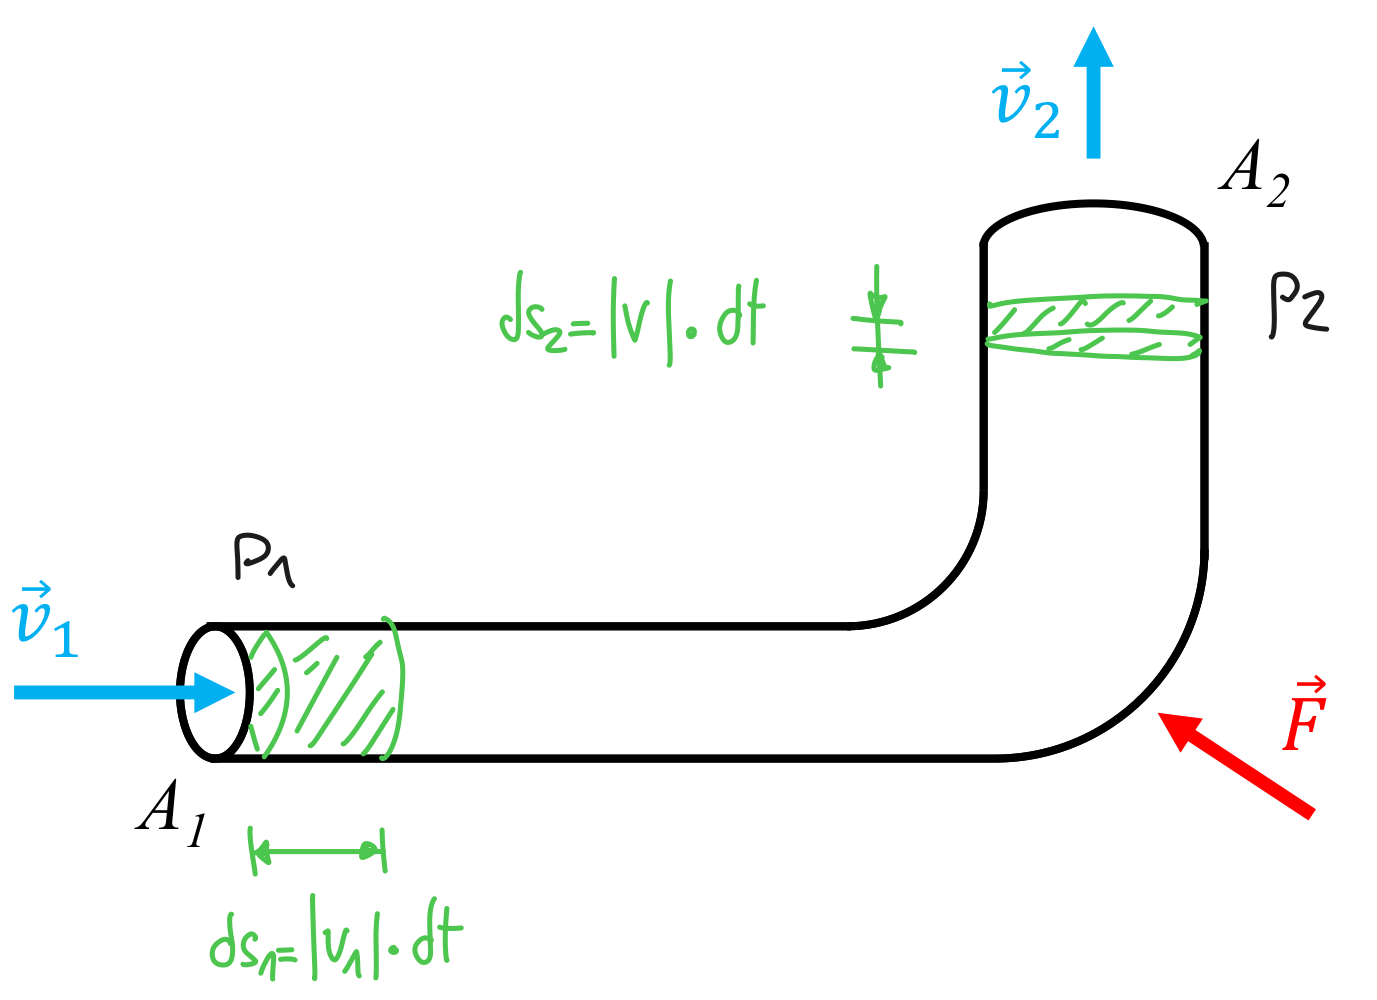
\includegraphics[width=\linewidth]{images/rohr_kraft.png}
\end{minipage}

\begin{center}
	\textit{le forze di pressione agiscono sempre verso l'interno del volume di controllo.} ($p \cdot A$)
\end{center}